%!Tex Root = ../main.tex
% ./Packete.tex
% ./Design.tex
% ./Deklarationen.tex
% ./Vorbereitung.tex
% ./Aufgabe1.tex
% ./Aufgabe2.tex
% ./Aufgabe4.tex
% ./Appendix.tex

\section{Aufgabe 3}

\setcounter{exercise}{1}

\begin{frame}[allowframebreaks]{Appendix}{CMOS, P-Kanal und N-Kanal Transistoren}

\begin{solutionnoinc}
\begin{table}
\tiny
\centering
\begin{tblr}{
  cells = {white},
  row{1} = {PrimaryColor,fg=white},
}
a & b & c & out \\
0 & 0 & 0 & 1   \\
0 & 0 & 1 & 0   \\
0 & 1 & 0 & 1   \\
0 & 1 & 1 & 0   \\
1 & 0 & 0 & 1   \\
1 & 0 & 1 & 0   \\
1 & 1 & 0 & 0   \\
1 & 1 & 1 & 0   
\end{tblr}
\caption{Wertetabelle for boolesche Funktion ${\overline{c}}\wedge({\overline{{a}}}\vee{\overline{{b}}})$}
\end{table}
\end{solutionnoinc}
\begin{solutionnoinc}
\begin{itemize}
    \item \alert{DNF:} $\overline{a}\overline{b}\overline{c} + \overline{a}b\overline{c} + a\overline{b}\overline{c}$
\end{itemize}
\alert{Karnaugh Map:} \begin{table}
\centering
\tiny
\begin{tblr}{
  cells = {white, c},
  row{1} = {PrimaryColor},
  cell{1}{2} = {fg=white},
  cell{1}{3} = {fg=white},
  cell{1}{4} = {fg=white},
  cell{1}{5} = {fg=white},
  cell{2}{2} = {SecondaryColorDimmed, fg=PrimaryColor},
  cell{2}{5} = {PrimaryColorDimmed},
  cell{3}{2} = {SecondaryColorDimmed},
  cell{2}{1} = {PrimaryColor,fg=white},
  cell{3}{1} = {PrimaryColor,fg=white},
}
\diagbox[linecolor=SecondaryColor]{\textcolor{white}{a}}{\textcolor{white}{bc}} & $\overline{b}\overline{c}$ & $\overline{b}c$ & $bc$ & $b\overline{c}$ \\
$\overline{a}$  & 1 & 0  &  0    &  1   \\
$a$  & 1 & 0  & 0  & 0    
\end{tblr}
\end{table}
\begin{itemize}
    \item \alert{Oder Webseite zur Hilfe nehmen:} \url{http://www.32x8.com/index.html}
\end{itemize}
\end{solutionnoinc}
\begin{solutionnoinc}
\begin{itemize}
    \item \alert{Vereinfachter Boolescher Ausdruck ($1$en):} $\overline{b}\overline{c}+\overline{a}\overline{c}$
\end{itemize}
\begin{table}
\tiny
\centering
\begin{tblr}{
  cells = {white, c},
  row{1} = {PrimaryColor,fg=white},
}
$a$ & $b$ & $c$ & $\overline{b}\overline{c}+\overline{a}\overline{c}$ \\
 0  &  0  &  0  & 1                                       \\
 0  &  0  &  1  & 0                                       \\
 0  &  1  &  0  & 1                                       \\
 0  &  1  &  1  & 0                                       \\
 1  &  0  &  0  & 1                                       \\
 1  &  0  &  1  & 0                                       \\
 1  &  1  &  0  & 0                                       \\
 1  &  1  &  1  & 0                                       
\end{tblr}
\end{table}
\end{solutionnoinc}
\begin{solutionnoinc}
\begin{itemize}
    \item \alert{KNF:} $(a+b+\overline{c}) \cdot (a+\overline{b}+\overline{c}) \cdot (\overline{a}+b+\overline{c})\cdot (\overline{a}+\overline{b}+c)\cdot(\overline{a}+\overline{b}+\overline{c})$
\end{itemize}
\alert{Karnaugh Map:} \begin{table}
\tiny
\centering
\begin{tblr}{
  cells = {white},
  column{3} = {SecondaryColorDimmed},
  column{4} = {SecondaryColorDimmed},
  row{1} = {PrimaryColor},
  column{1} = {PrimaryColor, fg=white},
  cell{1}{2} = {fg=white},
  cell{1}{3} = {fg=white},
  cell{1}{4} = {fg=white},
  cell{1}{5} = {fg=white},
  cell{3}{5} = {PrimaryColorDimmed},
  cell{3}{4} = {fg=PrimaryColor},
}
\diagbox[linecolor=SecondaryColor]{\textcolor{white}{a}}{\textcolor{white}{bc}} & $\overline{b}\overline{c}$ & $\overline{b}c$ & $bc$ & $b\overline{c}$ \\
$\overline{a}$  & 1 & 0  &  0    &  1   \\
$a$  & 1 & 0  & 0  & 0    
\end{tblr}
\end{table}
\end{solutionnoinc}
\begin{solutionnoinc}
\begin{itemize}
    \item \alert{Vereinfachter Boolescher Ausdruck ($0$en):} $c + ab$
    % \item \alert{Feststellung:} Der Ausdruck aus der Aufgabenstellung war bereits ein maximal reduzierter Ausdruck in KNF
\end{itemize}
\begin{table}
\tiny
\centering
\begin{tblr}{
  cells = {white, c},
  row{1} = {PrimaryColor,fg=white},
}
$a$ & $b$ & $c$ & $c + ab$ \\
 0  &  0  &  0  & 0                                       \\
 0  &  0  &  1  & 1                                       \\
 0  &  1  &  0  & 0                                       \\
 0  &  1  &  1  & 1                                       \\
 1  &  0  &  0  & 0                                       \\
 1  &  0  &  1  & 1                                       \\
 1  &  1  &  0  & 1                                       \\
 1  &  1  &  1  & 1                                       
\end{tblr}
\end{table}
\end{solutionnoinc}
\begin{solutionnoinc}
    \begin{itemize}
        \item auf der einen Seite mit den P-Kanal-Transistoren wird der vereinfachte Ausdruck umgesetzt, der für genau die Modelle wahr ist, für welche die logische Funktion $\overline{c}\cdot(\overline{a}+\overline{b})$ \alert{wahr} ist. 
        \item Auf der anderen Seite mit den N-Kanal Transistoren wird der vereinfachte Ausdruck umgesetzt, der für genau die Modelle wahr ist, für welche die logische Funktion $\overline{c}\cdot(\overline{a}+\overline{b})$ \alert{falsch} ist.
        \item damit wird sichergestellt, dass es zu keinem \alert{Kurzschluss} kommen kann, weil immer nur entweder die eine oder anderen Seite ein Signal $0$ (Ground) oder $1$ ($Vdd$) zu $out$ durchlässt, aber niemals beide, da der eine mit P-Kanal-Transistoren umgesetzte Ausdruck für genau die Modelle wahr ist, für die der andere mit N-Kanal-Transistoren umgesetzte Ausdruck falsch ist.
    \end{itemize}
\end{solutionnoinc}
\begin{solutionnoinc}
    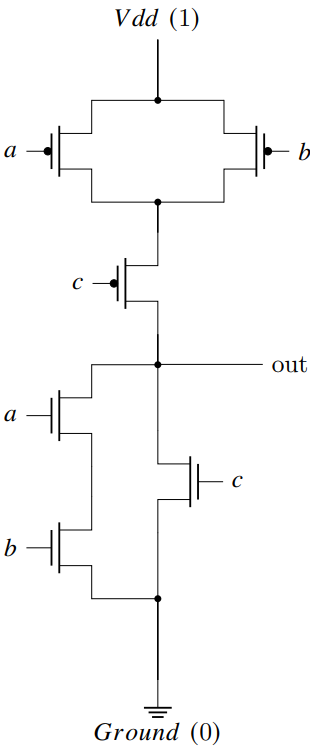
\includegraphics[height=0.6\textheight, center]{./figures/3.png}
\end{solutionnoinc}
\end{frame}

% \begin{frame}[allowframebreaks]{Appendix}{Euklidischer Algorithmus}
%     \begin{}
%     \begin{itemize}
%         \item asdf
%     \end{itemize}
% \end{frame}
